\section{ DOM}

\begin{frame}[fragile]{CH9 文档对象模型DOM}
\begin{figure}
    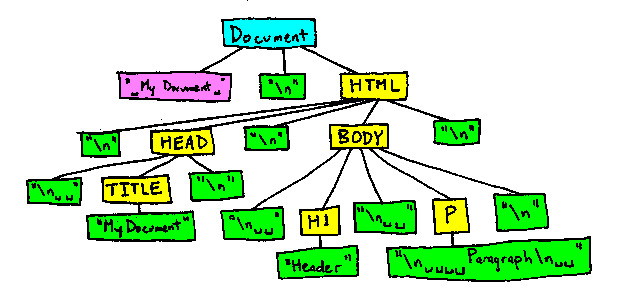
\includegraphics[width=0.9\textwidth]{figure/dom.png}
\end{figure}
\end{frame}

\begin{frame}[fragile]{本章学习目标}
\begin{easylist} \easyitem
& 了解DOM的特点及规范级别
& 掌握常见的DOM对象
& 熟悉浏览器操纵HTML文档和XML文档的基本方法
\end{easylist}
\end{frame}

\begin{frame}[fragile]{目录}
\begin{easylist} \easyitem
& DOM概述
& DOM基本对象
& 利用Mongoose搭建DOM测试环境
& 利用DOM操纵HTML
& 利用DOM操纵XML
\end{easylist}
\end{frame}


\subsection{9.1 DOM概述}

\begin{frame}[fragile]{9.1 DOM概述}
\begin{easylist} \easyitem
& DOM——Document Object Model
&& 文档对象模型的缩写,把整个XML文档表示成一棵由结点组成的层次树,方便人们通过编程语言进行操纵处理
&& 面向程序员实现对XML的操纵处理
\end{easylist}
\end{frame}


\begin{frame}[fragile]{DOM的优点}
\begin{easylist} \easyitem
& DOM优点
&& DOM以易于程序员理解的结点树表示XML文档,简化了文档操作
&& DOM提供了语言中立的标准接口,降低了学习和交流成本
& 其他处理技术
&& SAX:Simple API for XML
&& StAX:Streaming API for XML
\end{easylist}
\end{frame}


\begin{frame}[fragile]{DOM历史及其规范级别}
\begin{easylist} \easyitem
& DOM Level 0
& DOM Level 1
& DOM Level 2
& DOM Level 3
\end{easylist}
\end{frame}



\subsection{9.2 DOM基本对象}

\begin{frame}[fragile]{9.2 DOM基本对象}
\begin{table}[!hbp] 
\begin{tabular}{l|l}
\Xhline{1.3pt}
对象名称 & 描述\\ \Xhline{1.3pt}
Attr & 表示一个属性结点 \\ \hline
Document & 表示XML文档整体 \\ \hline
DocumentFragment & 表示一个XML文档片段结点 \\ \hline
DocumentType & 表示<!DOCTYPE> 元素结点 \\ \hline
Entity & 表示XML文档中的一个实体结点 \\ \hline
EntityReference & 表示XML文档中的一个实体引用结点 \\ \hline
Element & 表示XML文档中的一个元素结点 \\ \hline
NamedNodeMap & 由若干个属性名称和属性值构成的无序集合 \\ \hline
Node & 表示文档树中的任一个结点 \\ \hline
NodeList & 表示一组结点构成的有序列表 \\ \hline
Notation & 表示一个Notation结点 \\ \hline
ProcessingInstruction & 表示一个处理指令结点 \\ \hline
Text & 表示元素或属性的文本内容结点 \\ \hline
\end{tabular}
\end{table}
\end{frame}


\begin{frame}[fragile, allowframebreaks]{XML文档与DOM树}
\begin{lstlisting}[tabsize=8, basicstyle=\small\tt, language=XML]
<?xml version="1.0" encoding="UTF-8"?>
<!-- DOM Demo -->
<book>
    <info author="乔治•伽莫夫" isbn="978-7-03-010759-6"/>
    <title>从一到无穷大</title>
</book>
\end{lstlisting}
\newpage
\begin{figure}
    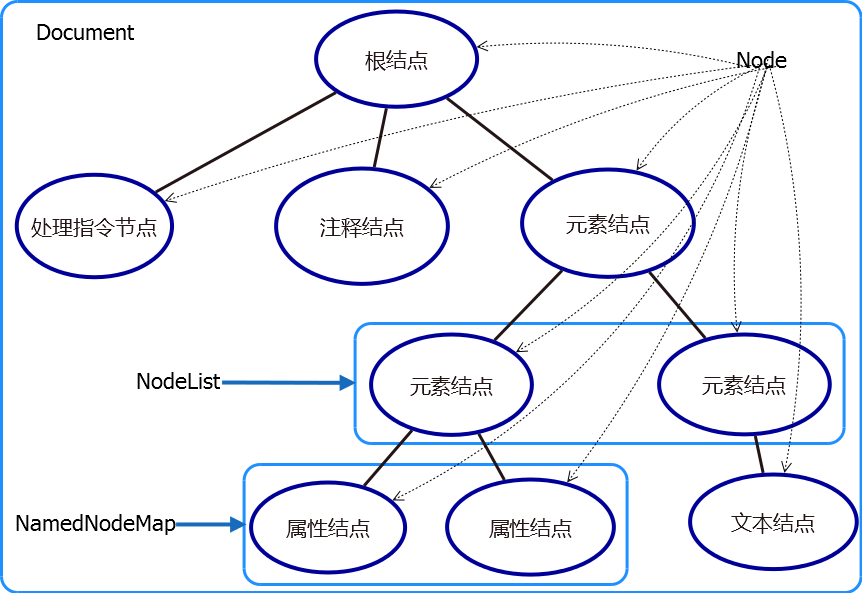
\includegraphics[width=0.9\textwidth]{figure/dom-object.png}
\end{figure}
\end{frame}



\subsection{9.3 利用Mongoose搭建DOM测试环境}

\begin{frame}[fragile]{9.3 利用Mongoose搭建DOM测试环境}
\begin{easylist} \easyitem
& Mongoose
&& 跨平台的Web服务器
& 为什么需要Web服务器
&& 访问拒绝错误
& 搭建步骤
&& 参考教材
\end{easylist}
\end{frame}


\begin{frame}[fragile]{利用浏览器访问本地搭建的Mongoose服务器}
\begin{figure}
    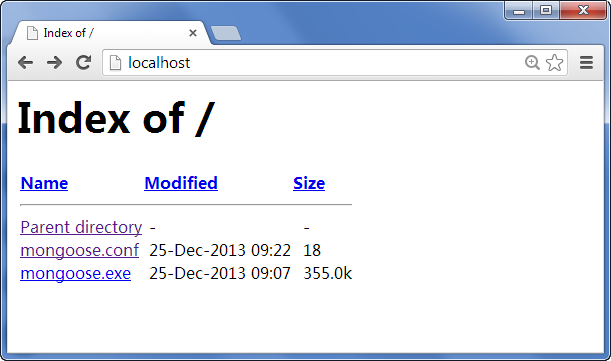
\includegraphics[width=0.9\textwidth]{figure/dom-mongoose.png}
\end{figure}
\end{frame}


\subsection{9.4 利用DOM操纵HTML}

\begin{frame}[fragile]{9.4 利用DOM操纵HTML}
\begin{easylist} \easyitem
& HTML DOM及元素定位方法
& 改变元素结点内容
& 改变属性结点内容
& 综合示例
\end{easylist}
\end{frame}


\subsubsection{9.4.1 HTML DOM及元素定位方法}
\begin{frame}[fragile, allowframebreaks]{9.4.1 HTML DOM及元素定位方法}
\begin{easylist} \easyitem
& HTML示例文档:
\begin{lstlisting}[tabsize=8, basicstyle=\small\tt, language=HTML]
<html>
    <head>
        <title>HTML DOM Example</title>
        <meta http-equiv="Content-Type" content="text/html;charset=utf-8" />
        <script type="text/javascript" src="jquery.js"></script>
    </head>
    <body id="main">
        <h1 id="headline">心情选择</h1>
        <div id="content">
            <span>今天的心情是:</span>
            <label for="happy_mood">开心</label>
            <input id="happy_mood" type="radio" name="mood" value="happy"/>
            <label for="bad_mood">心情不好</label>
            <input id="bad_mood" type="radio" name="mood" value="bad"/>
        </div>
    </body>
</html>
\end{lstlisting}
& HTML文档对于的HTML DOM树:
\begin{figure}
    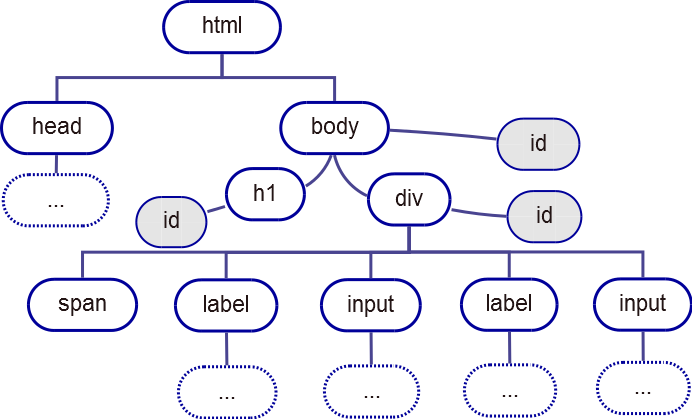
\includegraphics[width=0.75\textwidth]{figure/dom-html-tree.png}
\end{figure}
\end{easylist}
\end{frame}


\begin{frame}[fragile]{定位方法}
\begin{easylist} \easyitem
& getElementById方法
\begin{lstlisting}[tabsize=8, basicstyle=\small\tt, language=JavaScript, numbers=none]
document.getElementById("content");
\end{lstlisting}
& getElementsByName方法
\begin{lstlisting}[tabsize=8, basicstyle=\small\tt, language=JavaScript, numbers=none]
document.getElementsByTagName(“mood”);
\end{lstlisting}
& getElementsByTagName方法
\begin{lstlisting}[tabsize=8, basicstyle=\small\tt, language=JavaScript, numbers=none]
document.getElementsByTagName("h1");
\end{lstlisting}
& jQuery选择方法
\begin{lstlisting}[tabsize=8, basicstyle=\small\tt, language=JavaScript]
$('#content'); //选择id为content的元素
$('input[name="mood"]');  //选择名称为mood的所有input元素
$('h1');  //选择标签名称为h1的所有元素
\end{lstlisting}
\end{easylist}
\end{frame}



\subsubsection{9.4.2 改变元素结点内容}
\begin{frame}[fragile]{9.4.2 改变元素结点内容}
\begin{easylist} \easyitem
& innerText
\begin{lstlisting}[tabsize=8, basicstyle=\small\tt, language=JavaScript]
var headline = document.getElementById("headline");
headline.innerText = '天天好心情';
\end{lstlisting}
& innerHTML
\begin{lstlisting}[tabsize=8, basicstyle=\small\tt, language=JavaScript]
var headline = document.getElementById("headline");
headline.innerHTML = '<font color="red">天天好心情</font>';
\end{lstlisting}
& jQuery方式
\begin{lstlisting}[tabsize=8, basicstyle=\small\tt, language=JavaScript]
$('#headline').text('天天好心情');
$('#headline').html('<font color="red">天天好心情</font>');
\end{lstlisting}
\end{easylist}
\end{frame}


\subsubsection{9.4.3 改变属性结点内容}
\begin{frame}[fragile]{9.4.3 改变属性结点内容}
\begin{easylist} \easyitem
& 设置属性
&& getAttribute()
& 获取属性
&& getAttribute()
\begin{lstlisting}[tabsize=8, basicstyle=\small\tt, language=JavaScript]
var headline = document.getElementById("headline");
headline.setAttribute('style', 'color:red;');
headline.getAttribute('style');
\end{lstlisting}
& jQuery方式
\begin{lstlisting}[tabsize=8, basicstyle=\small\tt, language=JavaScript]
$('#headline').attr('style','color:red;');
$('#headline').attr('style');
\end{lstlisting}
\end{easylist}
\end{frame}


\subsubsection{9.4.4 结点的创建与删除}
\begin{frame}[fragile, allowframebreaks]{9.4.4 结点的创建与删除}
\begin{easylist} \easyitem
& 创建元素结点
&& createElement( )
& 把新创建的结点附加到特定结点内
&& appendChild( )
\begin{lstlisting}[tabsize=8, basicstyle=\small\tt, language=JavaScript]
var button = document.createElement("input");
button.setAttribute('id', 'guess_button');
button.setAttribute('type', 'button');
button.setAttribute('value', 'Guess');
var container = document.getElementById('content');
container.appendChild(button);
\end{lstlisting}
& 创建一个文本结点
&& createTextNode( )
\begin{lstlisting}[tabsize=8, basicstyle=\small\tt, language=JavaScript]
var textNode = document.createTextNode('静以修身');
container.appendChild(textNode);
\end{lstlisting}
& 删除结点
&& removeChild( )
\begin{lstlisting}[tabsize=8, basicstyle=\small\tt, language=JavaScript]
container.removeChild(textNode);
\end{lstlisting}
\end{easylist}
\end{frame}



\subsubsection{9.4.5 示例}
\begin{frame}[fragile, allowframebreaks]{9.4.5 示例}
\begin{easylist} \easyitem
& 代码清单
\begin{lstlisting}[tabsize=8, basicstyle=\small\tt, language=HTML]
<html>
    <head>
        <title>HTML DOM Example</title>
        <meta http-equiv="Content-Type" content="text/html;charset=utf-8" />
        <script type="text/javascript" src="jquery.js"></script>
        <script type="text/javascript">
            $(document).ready(function(){
                var headline = document.getElementById("headline");
                
                headline.innerText = '天天好心情'; 
                headline.innerHTML = '<font color="red">天天好心情</font>'; 
            
                $('#headline').text('天天好心情'); 
                $('#headline').html('<font color="red">天天好心情</font>'); 
                
                headline.setAttribute('style', 'color:red;'); 
                console.info(headline.getAttribute('style')); //获取h1的style属性值
                
                $('#headline').attr('style','color:red;'); 
                console.info($('#headline').attr('style')); //获取h1的style属性值
                
                var button = document.createElement("input");
                button.setAttribute('id', 'guess_button'); 
                button.setAttribute('type', 'button'); 
                button.setAttribute('value', 'Guess'); 
                var container = document.getElementById('content'); 
                container.appendChild(button);  //把创建的button结点附加到id为content的元素下
                
                var textNode = document.createTextNode('静以修身'); 
                container.appendChild(textNode); 
                
                container.removeChild(button); //删除结点
            });
        </script>
    </head>
    <body id="main">
        <h1 id="headline">心情选择</h1>
        <div id="content">
            <span>今天的心情是:</span>
            <label for="happy_mood">开心</label>
            <input id="happy_mood" type="radio" name="mood" value="happy"/>
            <label for="bad_mood">心情不好</label>
            <input id="bad_mood" type="radio" name="mood" value="bad"/>
        </div>
    </body>
</html>
\end{lstlisting}
& 显示效果
\begin{figure}
    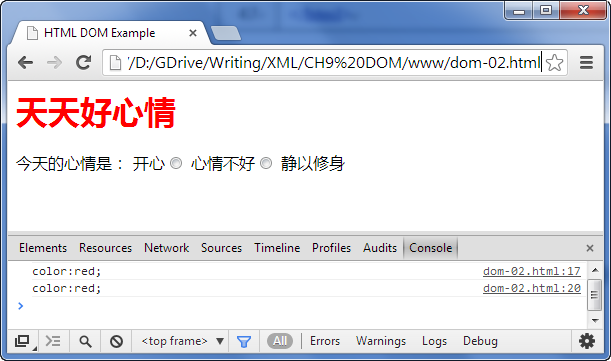
\includegraphics[width=0.75\textwidth]{figure/dom-html-display.png}
\end{figure}
\end{easylist}
\end{frame}



\subsection{9.5 利用DOM操纵XML}

\begin{frame}[fragile]{9.5 利用DOM操纵XML}
\begin{easylist} \easyitem
& 加载XML文档
& 结点访问方法
& 结点定位属性
& 结点常用属性
& 结点常用方法
& 示例
\end{easylist}
\end{frame}

\begin{frame}[fragile, allowframebreaks]{示例XML文档:books.xml}
\begin{lstlisting}[tabsize=8, basicstyle=\small\tt, language=XML]
<?xml version="1.0"?>
<books>
    <book isbn="978-1449319793" id=”b1”>
        <title lang="EN">Python for Data Analysis</title>
        <price currency="dollar">25.40</price>
        <authors>
            <author>Wes McKinney</author>
        </authors>
        <press> O'Reilly Media</press>
        <pages>470</pages>
        <description>Python for Data Analysis is concerned with the nuts…</description>
        <cover>book-python.jpg</cover>
    </book>
    <book isbn="978-7-115-28282-8" id=”b2”>
        <title lang="CHN">数学之美</title>
        <price>45.00</price>
        <authors>
            <author>吴军</author>
        </authors>
        <press>人民邮电出版社</press>
        <pages>304</pages>
        <description>读了“数学之美”,才发现大学时学的数学知识…</description>
        <cover>book-math.jpg</cover>
    </book>
</books>
\end{lstlisting}
\end{frame}


\subsection{9.5.1 加载XML文档}
\begin{frame}[fragile, allowframebreaks]{9.5.1 加载XML文档}
\begin{easylist} \easyitem
& XMLHttpRequest
&& IE7+、Firefox、Chrome、Safari以及Opera
&& 老版本的浏览器可能不支持
& 自定义的加载XML文档函数
\begin{lstlisting}[tabsize=8, basicstyle=\small\tt, language=JavaScript]
function loadXml(xmlFile) {
    var xhttp = new XMLHttpRequest();
    xhttp.open("GET", xmlFile, false); 
    xhttp.send();
    return xhttp.responseXML;
}
\end{lstlisting}
& XMLHttpRequest的open()
\begin{lstlisting}[tabsize=8, basicstyle=\small\tt, language=JavaScript, numbers=none]
void open(string method, string URL, boolean asynch, string username, string password);
\end{lstlisting}
&& method
&&& 向服务器发送请求的方式
&&& 可以为GET或POST
&& URL
&&& 所调用的服务器资源的URL
&& asynch
&&& 布尔值,说明调用时是异步方式还是同步方式
&&& 默认为true,即异步调用方式
&& username和password
&&& 在必要时指定访问资源所需要的用户名和口令
& XMLHttpRequest的send()
\begin{lstlisting}[tabsize=8, basicstyle=\small\tt, language=JavaScript, numbers=none]
void send(content);
\end{lstlisting}
&& 如open()方法中的asynch参数为true,send()方法就会立即返回
&& 否则它会等待,直到接收到响应为止
&& content是可选参数
& XMLHttpRequest的返回结果
&& responseXML 
&& responseText
\end{easylist}
\end{frame}

\begin{frame}[fragile]{利用DOMParser对象从字符串中加载XML}
\begin{lstlisting}[tabsize=8, basicstyle=\small\tt, language=JavaScript]
function loadXmlFromString(str) {
    var parser = new DOMParser();
    var xmlDoc = parser.parseFromString(str, "text/xml");
    return xmlDoc
}
\end{lstlisting}
\end{frame}


\subsection{9.5.2 结点访问方法}
\begin{frame}[fragile]{9.5.2 结点访问方法}
\begin{easylist} \easyitem
& 获取指定结点下指定标记名称的结点集合
\begin{lstlisting}[tabsize=8, basicstyle=\small\tt, language=JavaScript, numbers=none]
node.getElementsByTagName("tagname");
\end{lstlisting}
&& 返回结果为NodeList
&&& 可通过下标访问每一个结点
&&& 可通过length属性获取结点集合的大小
&&& 示例:
\begin{lstlisting}[tabsize=8, basicstyle=\small\tt, language=JavaScript]
var titleList = xmlDoc.getElementsByTagName("title");
for(var i=0; i<titleList.length; i++) {
    var titleNode = titleList[i]; 
    //其他处理
}
\end{lstlisting}
\end{easylist}
\end{frame}


\subsection{9.5.3 结点定位属性}
\begin{frame}[fragile]{9.5.3 结点定位属性}
\begin{easylist} \easyitem
& 从当前结点根据结点树关系进行访问
&& parentNode:返回当前结点的父节点。
&& childNodes:该属性用于获取当前结点的直接子结点集合,返回结果为NodeList对象,与getElementsByTagName()方法相同。
&& firstChild:返回当前结点的第一个孩子结点。
&& lastChild:返回当前结点的最后一个孩子结点。
&& nextSibling:返回当前结点的下一个兄弟结点。
&& previousSibling:返回当前结点的上一个兄弟结点。
\end{easylist}
\end{frame}

\begin{frame}[fragile]{示例}
\begin{lstlisting}[tabsize=8, basicstyle=\small\tt, language=JavaScript]
var firstBookNode = xmlDoc.getElementsByTagName('book')[0];
for(var node = firstBookNode.firstChild; 
        node!=null; 
        node = node.nextSibling) {
    console.info(node);
    if(node==firstBookNode.lastChild) break;
}
\end{lstlisting}
\end{frame}


\subsection{9.5.4 结点常用属性}
\begin{frame}[fragile]{9.5.4 结点常用属性}
\begin{easylist} \easyitem
& nodeName
& nodeValue
& nodeType
& attributes
\end{easylist}
\end{frame}

\begin{frame}[fragile]{nodeName}
\begin{easylist} \easyitem
& 元素结点的nodeName与标签名相同
& 属性结点的nodeName是属性的名称
& 文本结点的nodeName永远是“\#text”
& 文档结点的nodeName永远是“\#document”
\end{easylist}
\end{frame}

\begin{frame}[fragile]{nodeValue}
\begin{easylist} \easyitem
& 元素结点的nodeValue是undefined
& 文本结点的nodeValue是文本自身
& 属性结点的nodeValue是属性的值
\end{easylist}
\end{frame}

\begin{frame}[fragile]{nodeType}
\begin{table}[!hbp] 
\begin{tabular}{l|l|l}
\Xhline{1.3pt}
结点类型 & 常量字符串 & 数值表示结果\\ \Xhline{1.3pt}
元素结点 & ELEMENT\_NODE & 1 \\ \hline
属性结点 & ATTRIBUTE\_NODE & 2 \\ \hline
文本结点 & TEXT\_NODE & 3 \\ \hline
CDATA块结点 & CDATA\_SECTION\_NODE & 4 \\ \hline
实体引用结点 & ENTITY\_REFERENCE\_NODE & 5 \\ \hline
实体结点 & ENTITY\_NODE & 6 \\ \hline
处理指令结点 & PROCESSING\_INSTRUCTION\_NODE & 7 \\ \hline
注释结点 & COMMENT\_NODE & 8 \\ \hline
文档结点 & DOCUMENT\_NODE & 9 \\ \hline
文档类型结点 & DOCUMENT\_TYPE\_NODE & 10 \\ \hline
文档片段结点 & DOCUMENT\_FRAGMENT\_NODE & 11 \\ \hline
NOTATION结点 & NOTATION\_NODE & 12 \\ \hline
\end{tabular}
\end{table}
\end{frame}

\begin{frame}[fragile]{attributes}
\begin{easylist} \easyitem
& 如果当前结点是元素类型的结点,attributes包含了当前元素的所有属性信息,否则为null
& attributes类型:NamedNodeMap
&& 无序结点集合
\end{easylist}
\end{frame}



\subsection{9.5.5 结点常用方法}
\begin{frame}[fragile]{9.5.5 结点常用方法}
\begin{easylist} \easyitem
& appendChild
& cloneNode
& hasChildNodes
& createElement
& insertBefore
& removeChild
& replaceChild
\end{easylist}
\end{frame}


\subsection{9.5.6 完整示例}
\begin{frame}[fragile, allowframebreaks]{9.5.6 完整示例}
\begin{easylist} \easyitem
& 在浏览器中显示"books.xml"的主要文档结构
& dom-tree.js
\begin{lstlisting}[tabsize=8, basicstyle=\small\tt, language=JavaScript]
function loadXmlFromFile(xmlFile) {
    var xhttp = new XMLHttpRequest();
    xhttp.open("GET", xmlFile, false); 
    xhttp.send();
    return xhttp.responseXML; 
}

var buffer = '';
$(document).ready(function () {
    var xmlDoc = loadXmlFromFile('books.xml'); //加载xml文档
    showTree(xmlDoc, 0);    //调用showTree()函数,输出结点树
    $('#main').html(buffer); //替换网页内容
});

function showTree(node, depth) {
    //输出当前node结点的信息
    writeNode(node, depth); 
    
    //循环输出当前结点的子结点信息
    var child = node.firstChild; 
    for(var child=node.firstChild;child!=null; child = child.nextSibling){ 
        showTree(child, depth + 4); 
        if(child==node.lastChild) break; 
    }
}

function writeNode(node, depth){
    if(node.nodeType==3){ 
        //忽略文本结点
        return; 
    } else if(node.nodeType==9){ //文档结点
        //处理文档结点
        buffer = node.nodeName; 
    } else if(node.nodeType == 1) {
        //处理元素结点
        buffer = buffer + '<br/>'; 
        for(var d=0; d<depth; d++) 
            buffer = buffer + '+'; 
            
        buffer = buffer + node.nodeName; 
        
        //处理元素的属性
        var attributes = node.attributes; 
        if(attributes.length > 0) {
            buffer = buffer + '['; 
            for(var i=0; i<attributes.length; i++) {
                if(i>0) buffer = buffer + ', '; 
                var att = attributes[i]; 
                buffer = buffer + att.nodeName + '=' + att.nodeValue; 
            }
            buffer = buffer + '] ';
        }
    }
}
\end{lstlisting}
& dom-tree.html
\begin{lstlisting}[tabsize=8, basicstyle=\small\tt, language=HTML]
<html>
    <head>
        <title>HTML DOM Node Test</title>
        <meta http-equiv="Content-Type" content="text/html;charset=utf-8" />
        <script type="text/javascript" src="jquery.js"></script>
        <!-- 引用dom-tree.js, 调用编写的脚本文件 -->
        <script type="text/javascript" src="dom-tree.js"></script>
    </head>
    <body id="main"></body>
</html>
\end{lstlisting}
& 在浏览器中的运行结果
\begin{figure}
    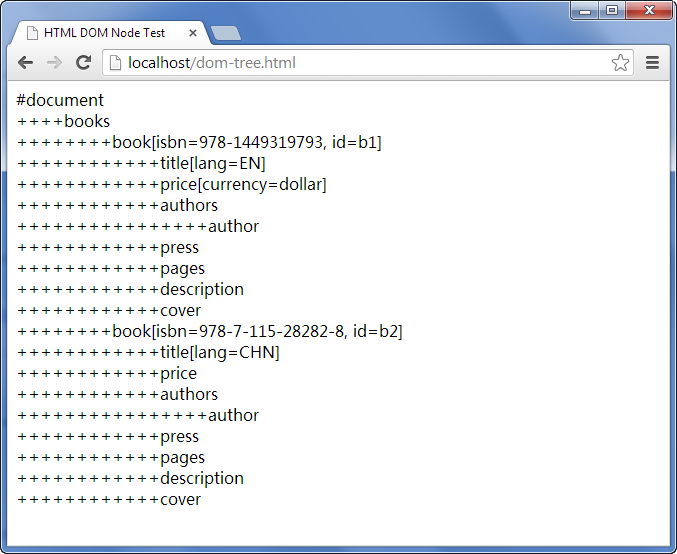
\includegraphics[width=0.75\textwidth]{figure/dom-tree.png}
\end{figure}
\end{easylist}
\end{frame}



\begin{frame}
\begin{center}
    \Huge END
\end{center}
\begin{figure}
    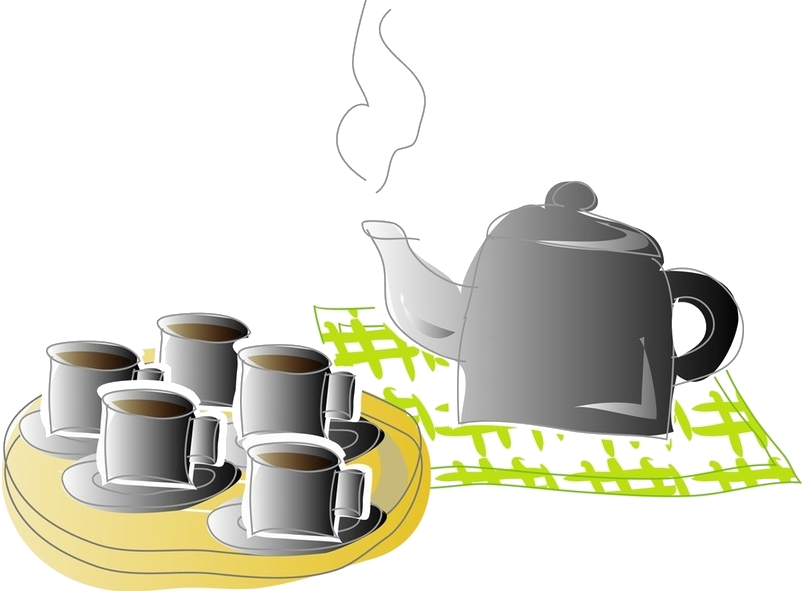
\includegraphics[width=0.75\textwidth]{figure/relax.png}
\end{figure}
\end{frame}
